\begin{figure*}[htbp]
\centering
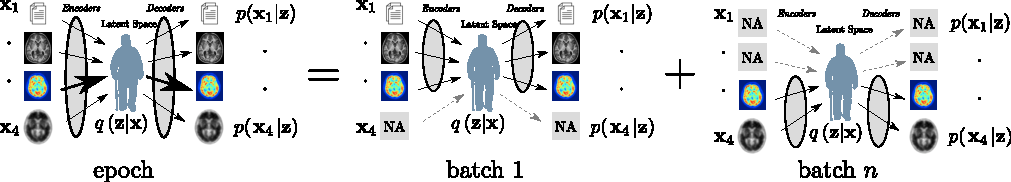
\includegraphics[width=\textwidth]{./tex/fig/model.pdf}
\caption{
Simple example of a Multi-view model learning scheme in the presence of missing not available (NA) data.
Arrows represent learnable functions used as network encoders and decoders, transforming respectively input views (\eg clinical scores, imaging derived phenotypes, \ldots) from the observation space to the latent space and from the latent space back to the observation space.
The separability of the loss function $\LBdnv$ in \eqnref{eq:newLB} allows to batch together observations into homogeneous groups.
For every batch, functions associated to missing views (dashed gray arrows) are locally not updated by the learning algorithm.
Globally, functions in common between couples of batches (thick arrows), being constrained to optimize multiple batches at the same time, act as a link allowing the information to flow throughout the views.
}
\label{fig:model}
\end{figure*}
